\documentclass[12pt,a4paper]{article}
\usepackage[utf8]{inputenc}
\usepackage[T1]{fontenc}
\usepackage{amsmath,amssymb,amsfonts}
\usepackage{graphicx}
\usepackage{booktabs}
\usepackage{hyperref}
\usepackage{natbib}
\usepackage[margin=1in]{geometry}
\usepackage{setspace}
\usepackage{caption}
\usepackage{float}

\onehalfspacing

\title{Currency Politics, Trade Conflict, and Exchange-Rate Exposure in the US--Japan Auto Industry: Evidence from LP-IV and Event Studies}
\author{So Kubota\\Tohoku University}
\date{September 23, 2026}

\begin{document}

\maketitle

\begin{abstract}
The US--Japan automobile relationship is a textbook case of how exchange rates, trade policy, and firm strategy co-evolve. In the 1980s, a weak Yen was widely viewed as a structural advantage for Japanese exporters, while US policymakers framed the bilateral auto trade deficit as evidence of unfair competition. Yet four decades of adaptation---voluntary export restraints (VERs), the Plaza Accord, repeated tariff threats, and the rise of ``transplant'' production in North America---have fundamentally changed where Japanese automakers produce, source, and earn.

This paper quantifies how that historical transformation maps into modern financial sensitivity. Using daily data for five major automakers (Toyota, Honda, Nissan, General Motors, Ford) and the USD/JPY exchange rate over a 10-year window, we estimate the dynamic causal effect of exchange-rate shocks on equity valuations with Local Projections Instrumental Variables (LP-IV). To address endogeneity between FX movements and equity returns, we instrument USD/JPY changes with innovations in the US 2-Year Treasury yield---a high-frequency proxy for monetary-policy surprises---while controlling for broad equity-market movements. The estimated impulse responses show sharp firm-level heterogeneity: GM and Nissan exhibit large positive cumulative responses to a 1\% USD/JPY appreciation shock (approximately $+18.3\%$ and $+22.6\%$ over 10 days), Honda and Ford show smaller but still positive responses ($+10.7\%$ and $+6.0\%$), while Toyota is uniquely insulated (terminal response $-0.24\%$, statistically indistinguishable from zero).

We triangulate the LP-IV results with an event study around eight major Bank of Japan and Federal Reserve policy shocks (2013--2024) that produced discrete jumps in USD/JPY. The event-study CARs replicate the same ranking: Toyota displays near-zero abnormal returns under both Yen appreciation and depreciation episodes, whereas Honda, Nissan, and the US firms show pronounced and often statistically significant reactions. We interpret these patterns through the lens of the US--Japan auto ``trade war'' and the strategic logic of operational hedging: deep localization of production and procurement can neutralize the macro-financial channel that once linked Yen movements to profitability.
\end{abstract}

\section{Introduction}

Few industries have been as central to the political economy of the US--Japan relationship as automobiles. Beginning in the 1970s, Japanese manufacturers gained US market share with smaller, more fuel-efficient vehicles, while Detroit specialized in larger cars and light trucks. As the bilateral trade imbalance widened, exchange rates became both an economic mechanism and a political symbol: a weak Yen was framed in Washington as a source of ``unfair'' export strength, and the auto deficit became a recurring object of negotiation.

The central empirical question of this paper is whether that classic narrative still holds in financial markets. If a Yen depreciation (a rise in USD/JPY) boosts Japanese exporters' competitiveness and translated profits, Japanese auto equities should rise when the Dollar strengthens against the Yen. Conversely, US auto firms should be harmed by a strong Dollar that compresses foreign earnings and weakens export competitiveness. Yet a long literature finds surprisingly weak reduced-form relationships between exchange rates and firm returns---the ``exchange-rate exposure puzzle'' \citep{bartram2010}. One reason is endogeneity: the same global shocks that move currencies also move equity risk premia.

A second reason is historical and structural. The era of ``Japan exports from Japan'' was progressively replaced by a North American production base. Under VERs in the early 1980s and especially after the Plaza Accord (1985) triggered a rapid Yen appreciation, Japanese automakers accelerated foreign direct investment into US assembly and parts capacity. Over time, localization became an operational hedge: revenues and costs were increasingly matched within the same currency area, weakening the link between USD/JPY and consolidated profits.

This paper contributes in three ways. First, it integrates the history of US--Japan auto trade conflict and currency diplomacy into the interpretation of modern exchange-rate exposure. Second, it estimates dynamic causal impulse responses using an LP-IV framework \citep{jorda2005} that is robust to model misspecification and explicitly addresses endogeneity. Third, it validates the time-series identification with a narrative event study \citep{mackinlay1997} around major BOJ/Fed policy surprises.

Our headline finding is stark: Toyota, the firm most associated with disciplined localization and supplier-system replication in North America, exhibits essentially zero equity sensitivity to USD/JPY shocks. Honda and Nissan remain meaningfully exposed, and the US manufacturers show positive exposure as well. The cross-firm ranking aligns with the depth of operational hedging induced by decades of trade friction.

The remainder of the paper is organized as follows. Section~2 reviews relevant literature. Section~3 provides a historically grounded account of the US--Japan auto ``trade war'' and the sequence of currency and trade-policy shocks that made localization strategically valuable. Section~4 describes the data and econometric design. Section~5 presents and interprets the empirical results in detail. Section~6 discusses implications for trade-policy narratives and corporate risk management. Section~7 concludes.

\section{Literature Review}

Research relevant to this paper spans four domains: (i) production systems and localization, (ii) trade conflict and currency politics in autos, (iii) exchange-rate exposure in financial economics, and (iv) econometric identification in macro-finance.

\paragraph{Lean production, transplants, and operational hedging.}

The operations literature explains why some Japanese firms could localize effectively while preserving quality and productivity. The ``lean production'' paradigm \citep{womack1990} formalized the Toyota Production System (TPS) as an alternative to mass production, emphasizing just-in-time logistics, continuous improvement, and tight supplier coordination. Detailed comparative work documented how Japanese production constraints and supplier relations shaped these systems \citep{cusumano1985,ohno1988}. For exchange-rate exposure, the key point is that lean production was not merely a factory technique: it was an organizational capability that could be replicated abroad, enabling the ``transplant'' strategy in North America \citep{rubenstein1992}. The depth of supplier localization varies by firm, implying heterogeneous operational hedging and, therefore, heterogeneous currency exposure.

\paragraph{US--Japan auto trade conflict, currency diplomacy, and pricing-to-market.}

The international-trade literature on autos highlights how policy constraints reshape firm behavior. The welfare and quality-upgrading effects of the early-1980s VERs were analyzed by \citet{feenstra1984}, who emphasized that quantity restrictions can induce compositional shifts toward higher-margin models. Currency diplomacy (especially the Plaza Accord) amplified pressure on Japanese exporters to move production offshore; narratives of this period emphasize the interaction between exchange-rate realignment and industrial adjustment \citep{funabashi1988}.

A complementary strand studies how firms adjust export prices and markups when exchange rates move (``pricing-to-market''), implying that the link between USD/JPY and profits depends on market structure and strategic pricing \citep{krugman1987,knetter1993,goldbergknetter1997}. In autos, the combination of imperfect competition and product differentiation means exchange-rate pass-through can be incomplete and state-dependent.

\paragraph{Exchange-rate exposure in equity returns.}

In finance, the canonical starting point is the definition of currency exposure in \citet{adler1984}. Empirically, many studies find weak or statistically insignificant exposure for most firms, despite theoretical predictions based on foreign-currency cash flows. \citet{bartram2010} systematized this evidence and labeled it the ``exchange-rate exposure puzzle.'' Proposed explanations include financial hedging with derivatives \citep{bodnar2002,allayannis2001} and operational hedging through global production networks \citep{pantzalis2001}. Our paper is closely related to the operational hedging mechanism but emphasizes that hedging is not uniform across firms, even within the same country and industry.

\paragraph{Causal identification in macro-finance: LP-IV and event studies.}

Our empirical design draws on modern time-series identification. Local projections \citep{jorda2005} estimate impulse responses flexibly without committing to a fully specified VAR. To address endogeneity, we use an instrumental-variables approach inspired by proxy-SVAR methods \citep{stock2012,mertens2013}, where high-frequency yield movements proxy for monetary-policy shocks that move exchange rates. We complement this continuous-time identification with an event-study design around discrete, well-documented BOJ and Fed announcements \citep{mackinlay1997}. The two approaches provide triangulation: they rely on different identifying variation but should agree if the underlying mechanism is stable.

\section{Institutional Background: Auto Trade War and Currency Politics}

The econometric patterns we document are best interpreted as outcomes of a long sequence of policy shocks and strategic responses. This section emphasizes how trade conflict and exchange-rate regimes shaped production localization, thereby altering exchange-rate exposure.

\paragraph{Divergent postwar industrial trajectories (1945--1970).}

After 1945 Japan rebuilt its industrial base under severe capital constraints and foreign-exchange scarcity. The Ministry of International Trade and Industry (MITI) actively nurtured strategic sectors, including automobiles, using protection, directed finance, and restrictions on foreign control \citep{johnson1982}. Domestic rivalry among Toyota, Nissan, and later Honda produced rapid learning under protection.

The US industry, by contrast, was mature and domestically oriented. Through the 1960s the ``Big Three'' dominated a large home market, and policy intervention was largely reactive. The institutional implication is that Japanese firms entered the 1970s with strong process discipline and a product mix suited to fuel efficiency, while US firms were optimized for a different domestic demand profile.

\paragraph{Oil shocks and the first surge of Japanese exports (1973--1980).}

The 1973 and 1979 oil shocks triggered a structural demand shift in the US toward smaller, fuel-efficient cars. Japanese models (e.g., Corolla, Civic) gained share rapidly, aided by perceived reliability and quality improvements linked to lean production. The speed of import penetration created an explicit political backlash in the US, including pressure from the United Auto Workers and congressional calls for protection.

\paragraph{The first ``trade war'': VERs, upgrading, and political economy (1981--1984).}

The Reagan administration pressed Japan into adopting voluntary export restraints in 1981, initially capping Japanese auto exports to the US at roughly 1.68 million units \citep{feenstra1984}. The VERs reshaped competition in two ways that matter for exchange-rate exposure.

First, constrained in quantity, Japanese producers raised average quality and price, effectively moving ``upmarket'' to protect margins. Second, the VERs increased the option value of producing inside the US: a car assembled in Ohio was not counted as an ``import'' and therefore bypassed the quota. These incentives set the stage for transplant investment even before the Plaza Accord.

\paragraph{Currency diplomacy and forced globalization: Plaza Accord to transplants (1985--1995).}

The Plaza Accord (September 1985) engineered a rapid Dollar depreciation. USD/JPY moved from around \textyen240 per Dollar in 1985 toward \textyen120 by 1987, implying a massive Yen appreciation and a direct shock to Japanese exporters' cost competitiveness. For automakers, this episode turned currency risk from a background variable into a strategic constraint.

The response was not simply financial hedging; it was a re-architecture of production. Honda's Marysville plant began in 1982, Nissan's Smyrna plant in 1983, and Toyota opened Georgetown, Kentucky in 1988. By the early 1990s, transplant assembly was large enough that an increasing share of ``Japanese'' cars sold in the US were produced in North America.

The critical margin for our empirical results is the \emph{depth} of localization. ``Localization'' can mean final assembly, but also local supplier development, engineering presence, and the replication of production routines. Toyota pushed furthest toward an integrated North American ecosystem, including the co-location of key suppliers and extensive process standardization. A firm that matches a large share of US Dollar revenues with US Dollar costs (wages, parts, logistics) has less exposure to USD/JPY movements.

\paragraph{Politics and the social meaning of the trade war.}

The auto dispute was not only about economics; it was a domestic political issue in both countries. In the United States, import penetration became intertwined with deindustrialization anxiety in the Midwest. ``Japan bashing'' in the 1980s included public demonstrations and symbolic acts such as the destruction of Japanese cars. The 1982 killing of Vincent Chin by laid-off autoworkers (who mistook him for Japanese) was an extreme and tragic manifestation of the period's tensions. These social dynamics mattered for firms because they increased the probability of abrupt policy intervention---quotas, tariffs, or local content rules---which made onshore production strategically valuable.

In Japan, the post-Plaza era of \textit{endaka} (a ``too-strong Yen'') created domestic pressure to protect employment while preserving export competitiveness. For automakers, overseas production could be framed as both a hedge against the exchange rate and a political response to US pressure: transplants reduced recorded imports and created US jobs, partially defusing protectionist threats.

\paragraph{The second ``trade war'': parts, non-tariff barriers, and the politics of the Yen (1995--2007).}

Even after transplants expanded, trade conflict persisted, shifting from finished vehicles toward market access, dealer networks, and auto parts procurement. US negotiators argued that Japanese distribution systems and supplier relations (\textit{keiretsu}) acted as non-tariff barriers. In the mid-1990s, negotiations repeatedly threatened punitive tariffs on Japanese luxury vehicles, while Japan emphasized that exchange-rate overvaluation (a ``strong Yen'') already constrained exporters.

The currency context matters: the mid-1990s also featured one of the strongest Yen episodes in the postwar period. A very strong Yen mechanically raised the Dollar price of Japan-based production and intensified pressure for pricing-to-market strategies. The pricing-to-market literature suggests that exporters in differentiated product markets often adjust markups to stabilize foreign-currency prices \citep{krugman1987,knetter1993}. In autos, incomplete pass-through implies that exchange-rate changes can show up as profit-margin variation rather than consumer price variation---which is precisely why investors may react to USD/JPY movements even when retail prices do not change one-for-one.

This period is also a transition: as local sourcing deepened, especially for Toyota and (to a somewhat lesser degree) Honda, the share of profits exposed to USD/JPY should decline. Firms with shallower supplier localization or more Japan-based production would retain higher exposure.

\paragraph{Global financial crisis, Abenomics, and renewed currency controversy (2008--2024).}

The 2008--2009 crisis and its aftermath re-centered exchange rates in macroeconomic debates. Safe-haven flows often strengthened the Yen during global stress, while unconventional BOJ policy and, later, Fed tightening cycles produced sharp interest-rate differentials. In the early 2010s, Japan's policy shift toward aggressive monetary easing (often associated with ``Abenomics'') coincided with a substantial Yen depreciation and renewed US political claims of competitive devaluation.

By this point, however, the transplant model had matured. Japanese automakers were no longer simply exporters; they were among the largest manufacturers in North America, employing US labor and buying from US-based suppliers. This blurs the traditional trade narrative: a weak Yen may raise the Yen value of repatriated profits, but it does not necessarily confer a simple price advantage in the US when production is local.

\paragraph{Firm case studies: why Toyota looks different.}

The empirical results later show Toyota as uniquely insulated from USD/JPY shocks. Historically, Toyota treated North America not as an ``export destination'' but as a second home production base. The strategy included (i) early learning through joint ventures (e.g., NUMMI), (ii) large-scale assembly investment (Georgetown and subsequent plants), and (iii) supplier co-location and capability transfer, often encouraging Japanese suppliers to build US capacity. Importantly, localization extended beyond assembly to engineering and procurement systems, allowing Toyota to stabilize both cost and quality. The result is a cash-flow structure in which Dollar revenues from US sales are matched by Dollar costs, dampening the earnings effect of USD/JPY moves.

Honda shares elements of this model, especially in its US manufacturing footprint, but its product mix and global allocation decisions differ. Nissan's US presence is also large, yet Nissan's later shift toward aggressive global cost-cutting and alliance-driven procurement reduced the stability of supplier relationships and, in some periods, increased reliance on imported components. These differences matter because operational hedging is not simply ``produce abroad''; it is the depth of the local ecosystem that determines how much of a firm's operating surplus is truly currency-matched.

\paragraph{A concise timeline of trade and currency episodes.}

Table~\ref{tab:timeline} summarizes key episodes linking trade policy, exchange-rate movements, and localization incentives.

\begin{table}[H]
\centering
\caption{Selected US--Japan auto trade and currency episodes and their strategic implications}
\label{tab:timeline}
\begin{tabular}{p{1.7cm} p{4.0cm} p{7.0cm}}
\toprule
Period & Episode & Exchange-rate / trade relevance for automakers \\
\midrule
1973--1980 & Oil shocks and import surge & US demand shifts to fuel-efficient cars; Japanese exports rise; political pressure for protection builds. \\
1981--1984 & Voluntary export restraints (VERs) & Quotas encourage quality upgrading and raise incentives to produce inside the US (transplants). \\
1985--1987 & Plaza Accord and rapid Yen appreciation & Currency shock compresses exporter margins; accelerates foreign production and supplier localization as an operational hedge. \\
1994--1995 & Market access and parts disputes & Trade conflict shifts to non-tariff barriers and parts sourcing; highlights strategic role of \textit{keiretsu} and localization depth. \\
2008--2012 & Global crisis and strong Yen episodes & Yen strength pressures Japan-based production; reinforces value of matching revenues and costs locally. \\
2013--2016 & BOJ QQE / NIRP and FX volatility & Large discrete USD/JPY moves become focal events for markets; firms with residual export dependence remain exposed. \\
2022--2024 & Fed--BOJ policy divergence & Interest-rate differentials drive USD/JPY swings; provides identification for our event study and IV strategy. \\
\bottomrule
\end{tabular}
\end{table}

\paragraph{Historical equity performance (10-year window).}
Against this institutional backdrop, the trailing-decade equity performance of the five firms diverges sharply, reflecting both firm-specific restructurings and macro regimes.

\begin{table}[H]
\centering
\caption{Summary statistics of equity performance (10-year sample)}
\begin{tabular}{lrrrr}
\toprule
Company & Total Return (\%) & Annual Return (\%) & Volatility (\%) & Max Drawdown (\%) \\
\midrule
GM (US) & 241.93 & 13.11 & 36.68 & $-59.96$ \\
Toyota (Japan) & 194.24 & 11.42 & 23.53 & $-36.80$ \\
Ford (US) & 88.78 & 6.57 & 36.64 & $-64.77$ \\
Honda (Japan) & 52.77 & 4.34 & 25.37 & $-43.12$ \\
Nissan (Japan) & $-67.07$ & $-10.53$ & 32.74 & $-80.91$ \\
\bottomrule
\end{tabular}
\end{table}

\begin{figure}[H]
\centering
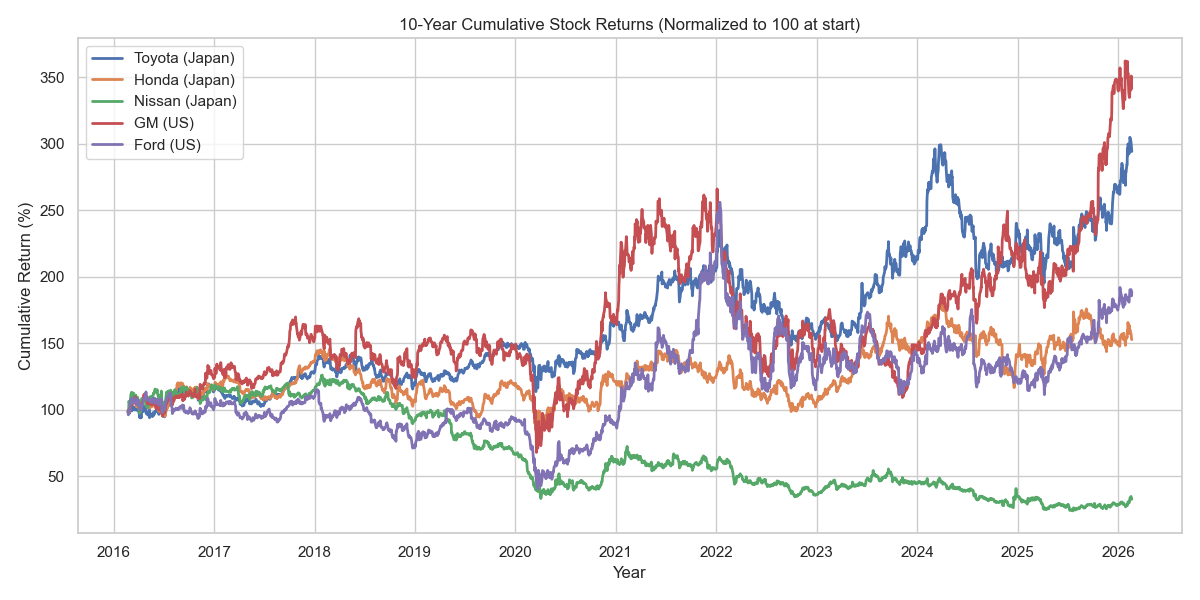
\includegraphics[width=0.9\textwidth]{cumulative_returns.png}
\caption{Cumulative equity returns normalized to 100 at the start of the sample. The patterns reflect both macro regimes and firm-specific turning points (notably Nissan's prolonged decline).}
\end{figure}

Toyota exhibits comparatively low volatility and a strong compounding trajectory, consistent with the view that operational discipline and localization dampen macro shocks. Nissan's negative decade-long performance and extreme drawdown reflect governance turmoil and strategic instability, which can amplify sensitivity to macro-financial variables, including exchange rates.

\section{Econometric Methodology}

To estimate the causal effect of exchange-rate shocks on equity valuations, we deploy two complementary approaches: (i) Local Projections with Instrumental Variables (LP-IV) to trace dynamic impulse responses, and (ii) an event study around discrete BOJ/Fed surprises.

\paragraph{Data.}

The dataset comprises daily observations over a 10-year horizon. Equity closing prices for Toyota, Honda, Nissan, GM, and Ford; the S\&P~500 index (\^{}GSPC); and the USD/JPY spot rate (JPY=X) are sourced from Yahoo Finance. The instrument---the daily change in the US 2-Year Treasury constant maturity yield (DGS2)---is sourced from FRED. Equity and exchange-rate series are converted to daily log returns; the 2-year yield is differenced (basis-point changes).

\paragraph{Interpreting an ``USD/JPY appreciation'' shock.}

Throughout, an ``appreciation'' shock refers to a positive change in USD/JPY (more Yen per Dollar). Economically, this is a \emph{Dollar appreciation and Yen depreciation}. Under the classic export model, a higher USD/JPY should benefit Japanese producers by improving price competitiveness and increasing the Yen value of Dollar revenues. Under deep localization, the effect should be smaller because costs and revenues are matched in the same currency area.

For US producers, the sign is theoretically ambiguous. A stronger Dollar can reduce the cost of imported inputs and foreign production expenses, but can also compress translated foreign earnings and weaken export competitiveness. Our empirical results therefore speak to the \emph{net} effect of a monetary-policy-induced USD/JPY move.

\paragraph{Endogeneity and the need for an instrument.}

A naive OLS regression of stock returns on USD/JPY changes is biased due to (i) reverse causality (equity risk-off episodes can generate safe-haven Yen appreciation) and (ii) omitted global shocks (risk appetite, commodity price changes, macro news) that jointly move both equities and exchange rates.

\paragraph{LP-IV specification.}

We estimate impulse responses over horizons $h \in \{0,1,\ldots,10\}$ using a two-stage least squares local-projections design \citep{jorda2005}.

\paragraph{First stage.} We instrument the endogenous USD/JPY return $X_t$ with the daily change in the US 2-year yield $Z_t$, controlling for the S\&P~500 return $W_t$:
\begin{equation}
X_t = \alpha_0 + \alpha_1 Z_t + \alpha_2 W_t + \nu_t.
\end{equation}
The fitted values $\widehat{X}_t$ capture exchange-rate variation plausibly driven by monetary-policy surprises, rather than contemporaneous equity shocks.

\paragraph{Second stage.} For each horizon $h$, we regress the cumulative return of firm $i$ from $t-1$ to $t+h$, denoted $Y_{t,t+h}$, on $\widehat{X}_t$ and $W_t$:
\begin{equation}
Y_{t,t+h} = \beta_{0,h} + \beta_{1,h} \widehat{X}_t + \beta_{2,h} W_t + \epsilon_{t+h}.
\end{equation}
The sequence $\{\beta_{1,h}\}$ traces the cumulative equity response to a 1\% USD/JPY appreciation shock.

\paragraph{Inference.} Because cumulative returns overlap across horizons, errors are serially correlated. We therefore use HAC (Newey--West) standard errors with the lag length scaled to $h+1$.

\paragraph{Event-study design and shock selection.}

As an external validation, we conduct a standard market-model event study \citep{mackinlay1997} around eight BOJ and Fed announcements (2013--2024) associated with large, discrete USD/JPY moves. ``Normal'' returns are estimated over an 110-trading-day window $[-120,-10]$, and abnormal returns (AR) and cumulative abnormal returns (CAR) are computed over an event window $[-1,+5]$.

The events are chosen because they generated prominent, sudden re-pricing in FX markets and were widely interpreted as surprises.

\paragraph{Yen depreciation episodes (USD/JPY jumps up).}
\begin{enumerate}
\item \textbf{April 4, 2013 -- BOJ ``QQE Bazooka''}: Governor Kuroda announced quantitative and qualitative easing far beyond expectations.
\item \textbf{October 31, 2014 -- BOJ expansion}: Surprise increase in asset purchases, reinforcing ``Abenomics''-era easing.
\item \textbf{August 26, 2022 -- Fed Jackson Hole}: Chairman Powell signaled an aggressive anti-inflation stance; yields rose and USD strengthened.
\item \textbf{March 19, 2024 -- BOJ exit from NIRP/YCC}: The BOJ ended negative rates; the Yen weakened as markets ``sold the news.''
\end{enumerate}

\paragraph{Yen appreciation episodes (USD/JPY drops).}
\begin{enumerate}
\item \textbf{January 29, 2016 -- BOJ NIRP}: Negative rates triggered paradoxical safe-haven flows and Yen appreciation.
\item \textbf{September 21, 2016 -- BOJ YCC}: Introduction of yield curve control, interpreted as a shift in the policy regime.
\item \textbf{December 20, 2022 -- BOJ YCC tweak}: Surprise widening of the YCC band, prompting a sharp Yen appreciation.
\item \textbf{July 28, 2023 -- BOJ YCC flexibility}: Increased tolerance for higher long yields, interpreted as de facto tightening.
\end{enumerate}

Table~\ref{tab:events} summarizes the event set.

\begin{table}[H]
\centering
\caption{BOJ/Fed policy events used in the narrative event study}
\label{tab:events}
\begin{tabular}{p{2.2cm} p{2.8cm} p{2.4cm} p{6.1cm}}
\toprule
Date & Institution & FX direction & Interpretation for USD/JPY \\
\midrule
2013-04-04 & BOJ & Depreciation & Major easing surprise; USD/JPY up (Yen down). \\
2014-10-31 & BOJ & Depreciation & Additional easing; USD/JPY up. \\
2016-01-29 & BOJ & Appreciation & NIRP backfired; risk-off dynamics strengthened Yen. \\
2016-09-21 & BOJ & Appreciation & YCC regime shift; Yen strengthened in the short run. \\
2022-08-26 & Fed & Depreciation & Hawkish signal; yields rose; USD strengthened. \\
2022-12-20 & BOJ & Appreciation & YCC band widening; Yen appreciated sharply. \\
2023-07-28 & BOJ & Appreciation & Greater YCC flexibility; interpreted as tightening. \\
2024-03-19 & BOJ & Depreciation & End of NIRP; Yen weakened on ``sell-the-news.'' \\
\bottomrule
\end{tabular}
\end{table}

\section{Empirical Results}

\paragraph{Descriptive co-movement and the reduced-form ``exposure puzzle''.}

We begin with a simple but revealing fact: unconditional correlations between daily equity returns and USD/JPY changes are close to zero for all five firms.

\begin{figure}[H]
\centering
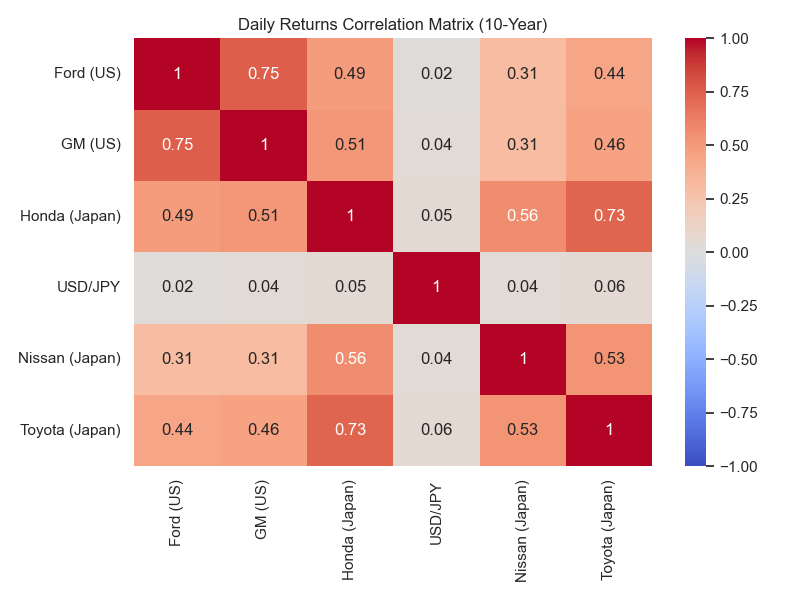
\includegraphics[width=0.75\textwidth]{correlation_matrix.png}
\caption{Pearson correlation matrix of daily returns (automakers and USD/JPY). USD/JPY correlations with equities are near zero, despite strong correlations within peer groups (e.g., Ford--GM and Honda--Toyota).}
\end{figure}

Two patterns stand out. First, co-movement is strongest within the US pair (Ford--GM correlation $0.75$) and within the Japanese set (Honda--Toyota correlation $0.73$; Nissan--Toyota $0.53$; Honda--Nissan $0.56$). Second, the USD/JPY correlations are tiny: between $0.02$ and $0.06$.

For transparency, Table~\ref{tab:fxcorr} reports the correlations between each automaker and USD/JPY.

\begin{table}[H]
\centering
\caption{Unconditional correlations between daily equity returns and USD/JPY}
\label{tab:fxcorr}
\begin{tabular}{lr}
\toprule
Firm & Corr$(r_{i,t},\Delta \log(USD/JPY)_t)$ \\
\midrule
Ford & 0.02 \\
GM & 0.04 \\
Honda & 0.05 \\
Nissan & 0.04 \\
Toyota & 0.06 \\
\bottomrule
\end{tabular}
\end{table}

If one interpreted these correlations literally, exchange rates would appear irrelevant for auto equities. This is misleading because daily exchange-rate changes mix many shocks. A Yen appreciation associated with global risk aversion, for example, can coincide with falling auto equities even if a pure currency translation shock would have the opposite sign. Causal identification therefore requires isolating a specific source of exogenous FX variation.

\paragraph{LP-IV impulse responses: heterogeneous and persistent FX sensitivity.}

Figure~\ref{fig:lpiv} reports LP-IV impulse responses to a 1\% USD/JPY appreciation (Dollar up / Yen down).

\begin{figure}[H]
\centering
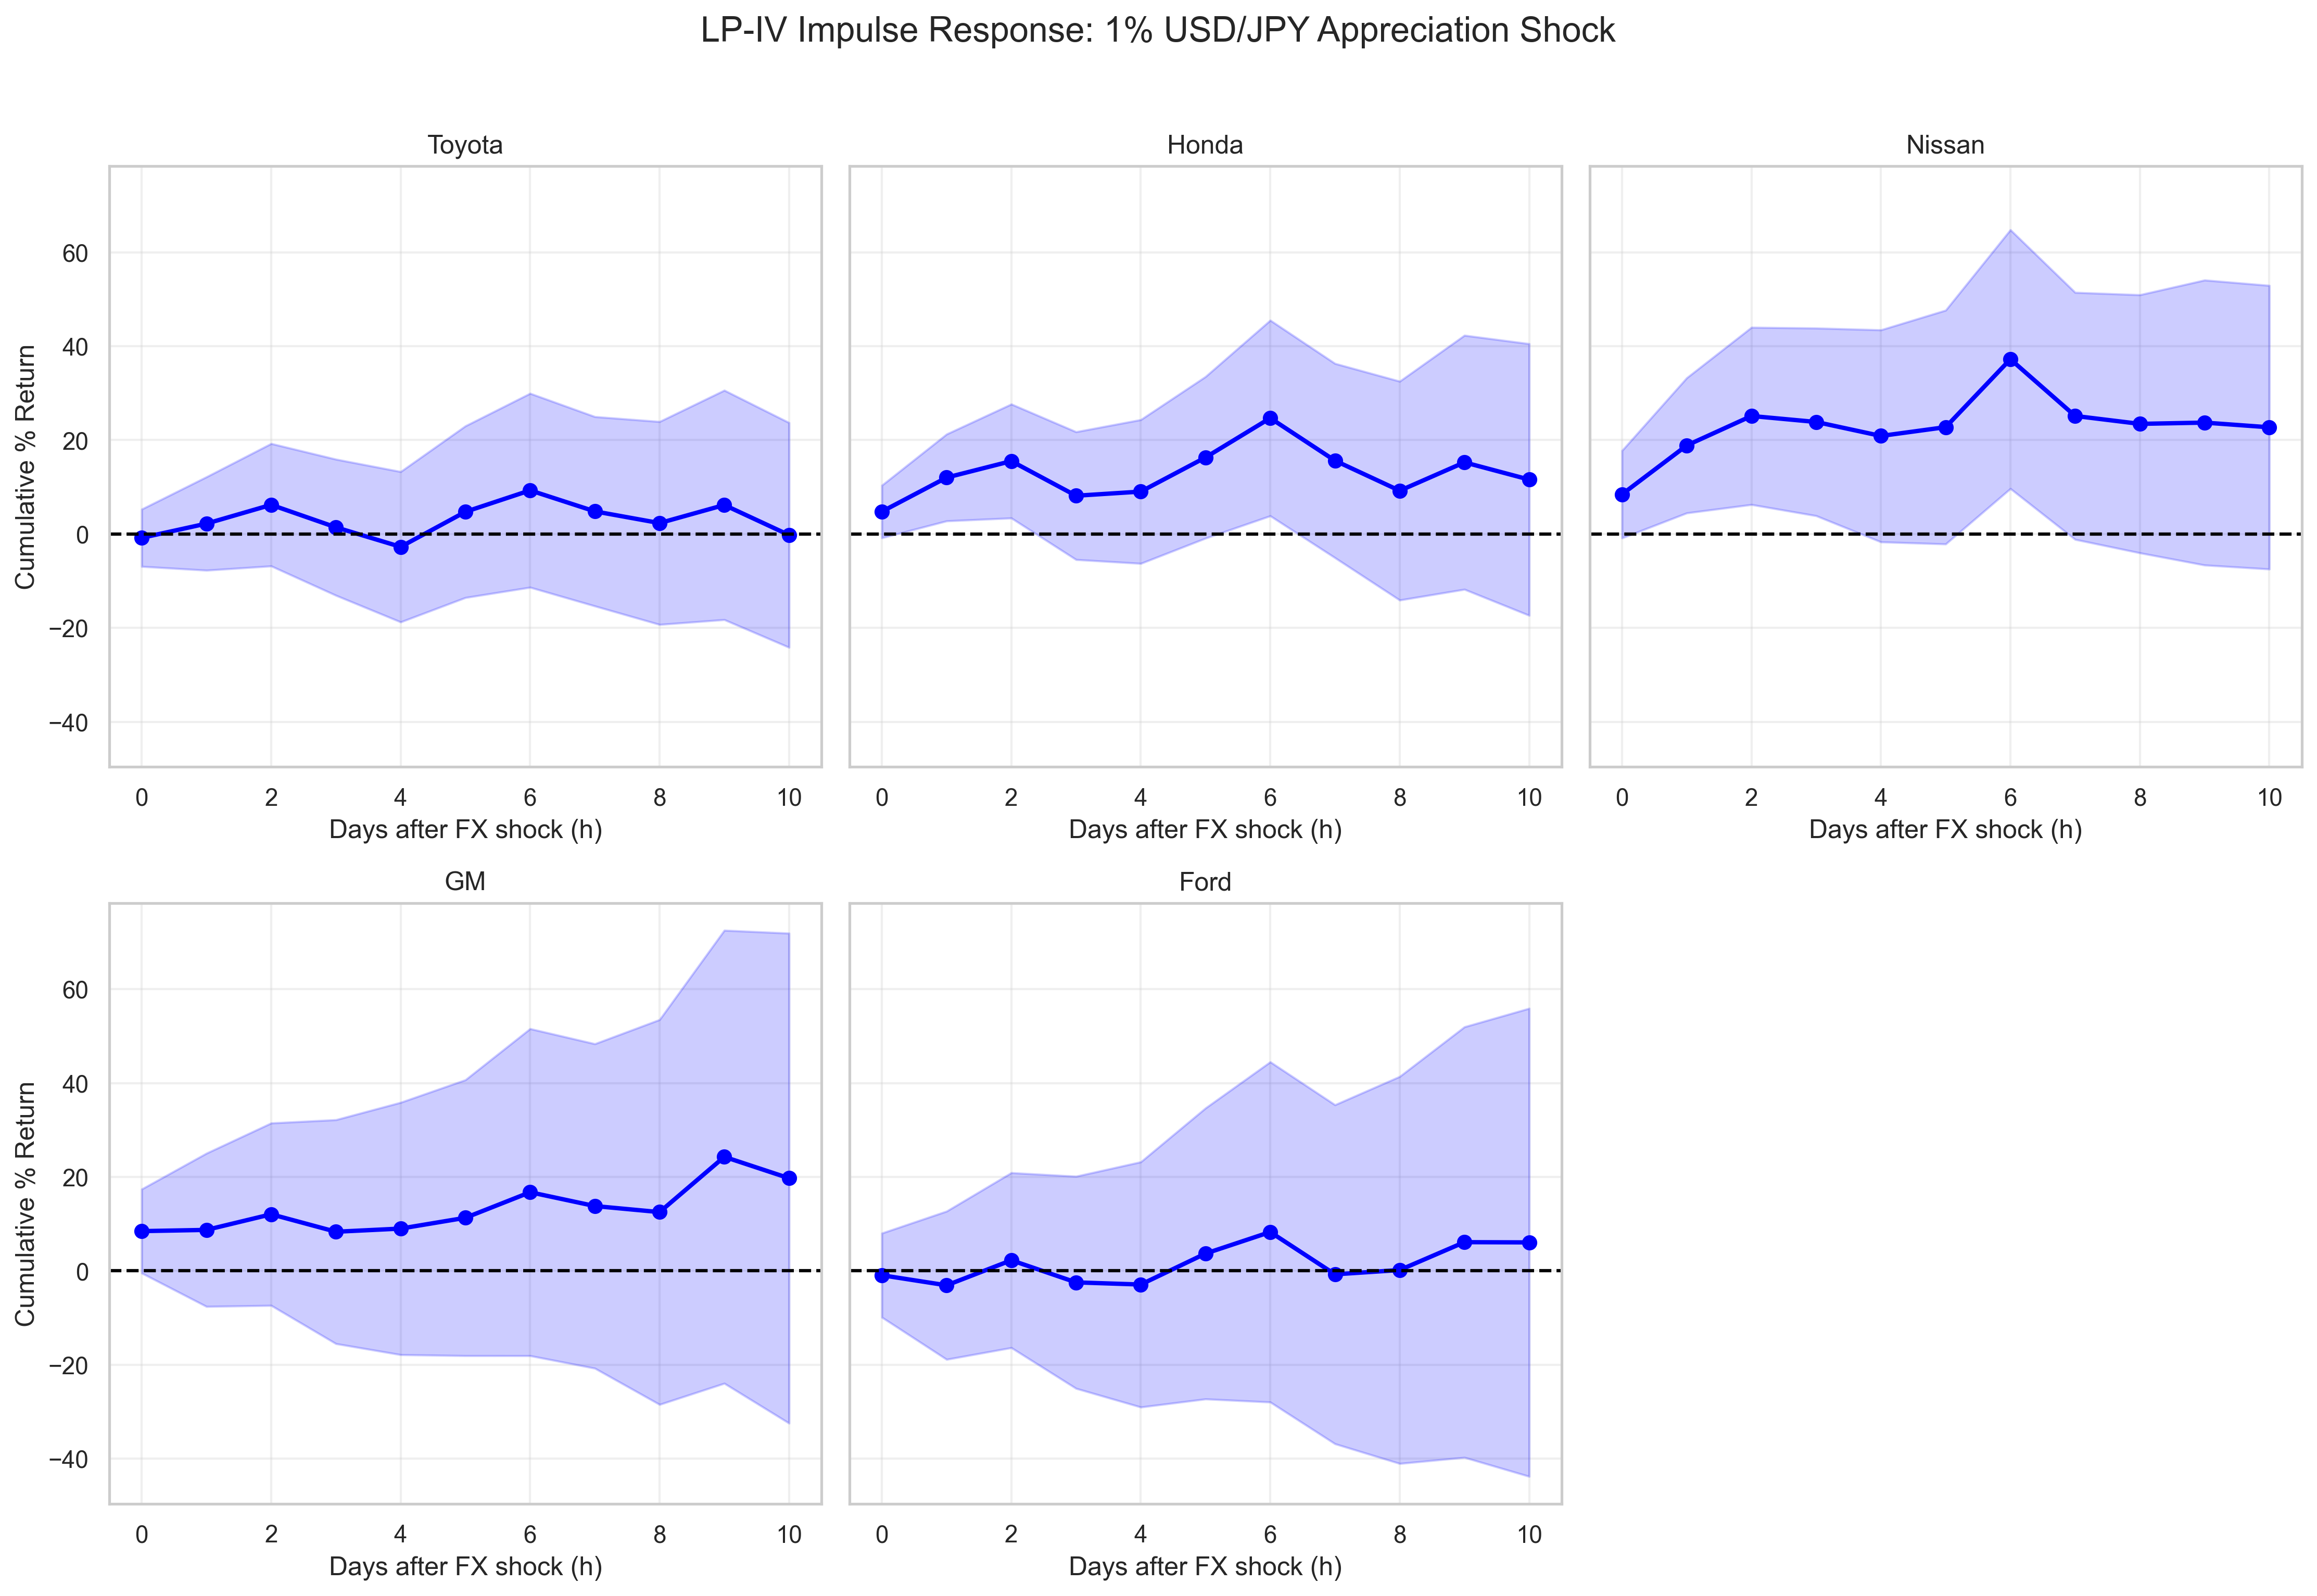
\includegraphics[width=0.9\textwidth]{lp_iv_irf.png}
\caption{LP-IV impulse responses to a 1\% USD/JPY appreciation shock. Shaded regions denote 95\% HAC-robust confidence intervals.}
\label{fig:lpiv}
\end{figure}

The impulse responses overturn the reduced-form correlation result. Four firms display economically large positive responses over horizons of one to two trading weeks, while Toyota remains essentially flat.

To summarize the cross-sectional ranking, Table~\ref{tab:lpivsummary} reports the terminal cumulative response at $h=10$.

\begin{table}[H]
\centering
\caption{LP-IV cumulative response to a 1\% USD/JPY appreciation shock at $h=10$}
\label{tab:lpivsummary}
\begin{tabular}{lr}
\toprule
Firm & Cumulative response (\%) \\
\midrule
Toyota & $-0.24$ \\
Ford & $+6.0$ \\
Honda & $+10.7$ \\
GM & $+18.3$ \\
Nissan & $+22.6$ \\
\bottomrule
\end{tabular}
\end{table}

\paragraph{Toyota: the benchmark case of operational insulation.}
Toyota's response oscillates around zero throughout the 10-day horizon, with a terminal estimate of $-0.24\%$ that is statistically indistinguishable from zero. This is consistent with ``deep localization'': if North American sales are largely produced and sourced in North America, Dollar revenues are naturally hedged by Dollar costs. In that case, a Dollar--Yen movement changes the accounting translation of some profits, but does not materially change expected operating cash flows.

\paragraph{Honda and Nissan: residual exposure under partial localization.}
Honda and Nissan display clear positive responses, with terminal cumulative effects of about $+10.7\%$ and $+22.6\%$. The point estimates suggest that a monetary-policy-driven Yen depreciation is interpreted by markets as a profit-positive shock for these firms. Historically, both firms localized production in the US, but with differences in supplier depth, product mix, and global footprint; the LP-IV results are consistent with the view that their consolidated earnings still contain a larger unmatched component exposed to currency translation and competitive pricing effects.

\paragraph{GM and Ford: positive responses despite an ambiguous theoretical sign.}
GM and Ford also show positive cumulative responses. This highlights that the relevant object is not ``currency exposure'' in a purely accounting sense, but the causal effect of a \emph{monetary-policy-induced} USD/JPY appreciation on equity values. Several channels can rationalize a positive sign: cheaper imported inputs, improved expected margins on foreign production when local costs fall in Dollar terms, and the possibility that yield-driven Dollar strength correlates with macro news that disproportionately affects cyclical industries.

\paragraph{Timing and persistence.}
The responses are not purely contemporaneous; they build over several days. For Nissan, the cumulative response grows quickly in the first week and remains elevated. For GM, the response increases more gradually and peaks later. Such timing is consistent with an earnings-expectations channel: exchange-rate news first alters expected margins and translation, and equity prices incorporate those revisions over several sessions.

\paragraph{Magnitude and uncertainty.}
The point estimates are large, especially for Nissan and GM. At longer horizons, confidence intervals widen substantially, reflecting overlapping-return estimation noise and the fact that confounding shocks accumulate over time even after instrumentation. Two implications follow. First, the cross-firm \emph{ranking} is more robust than any single horizon's precise magnitude: Toyota is consistently least sensitive, Nissan and GM most sensitive. Second, the responses should be interpreted as the effect of a particular class of FX movements (those induced by short-rate surprises) rather than a universal mapping from any USD/JPY fluctuation to equity returns.

\paragraph{Event-study evidence: discrete policy shocks and asymmetric CARs.}
The event study provides a narrative check using discrete BOJ/Fed surprises.

\begin{figure}[H]
\centering
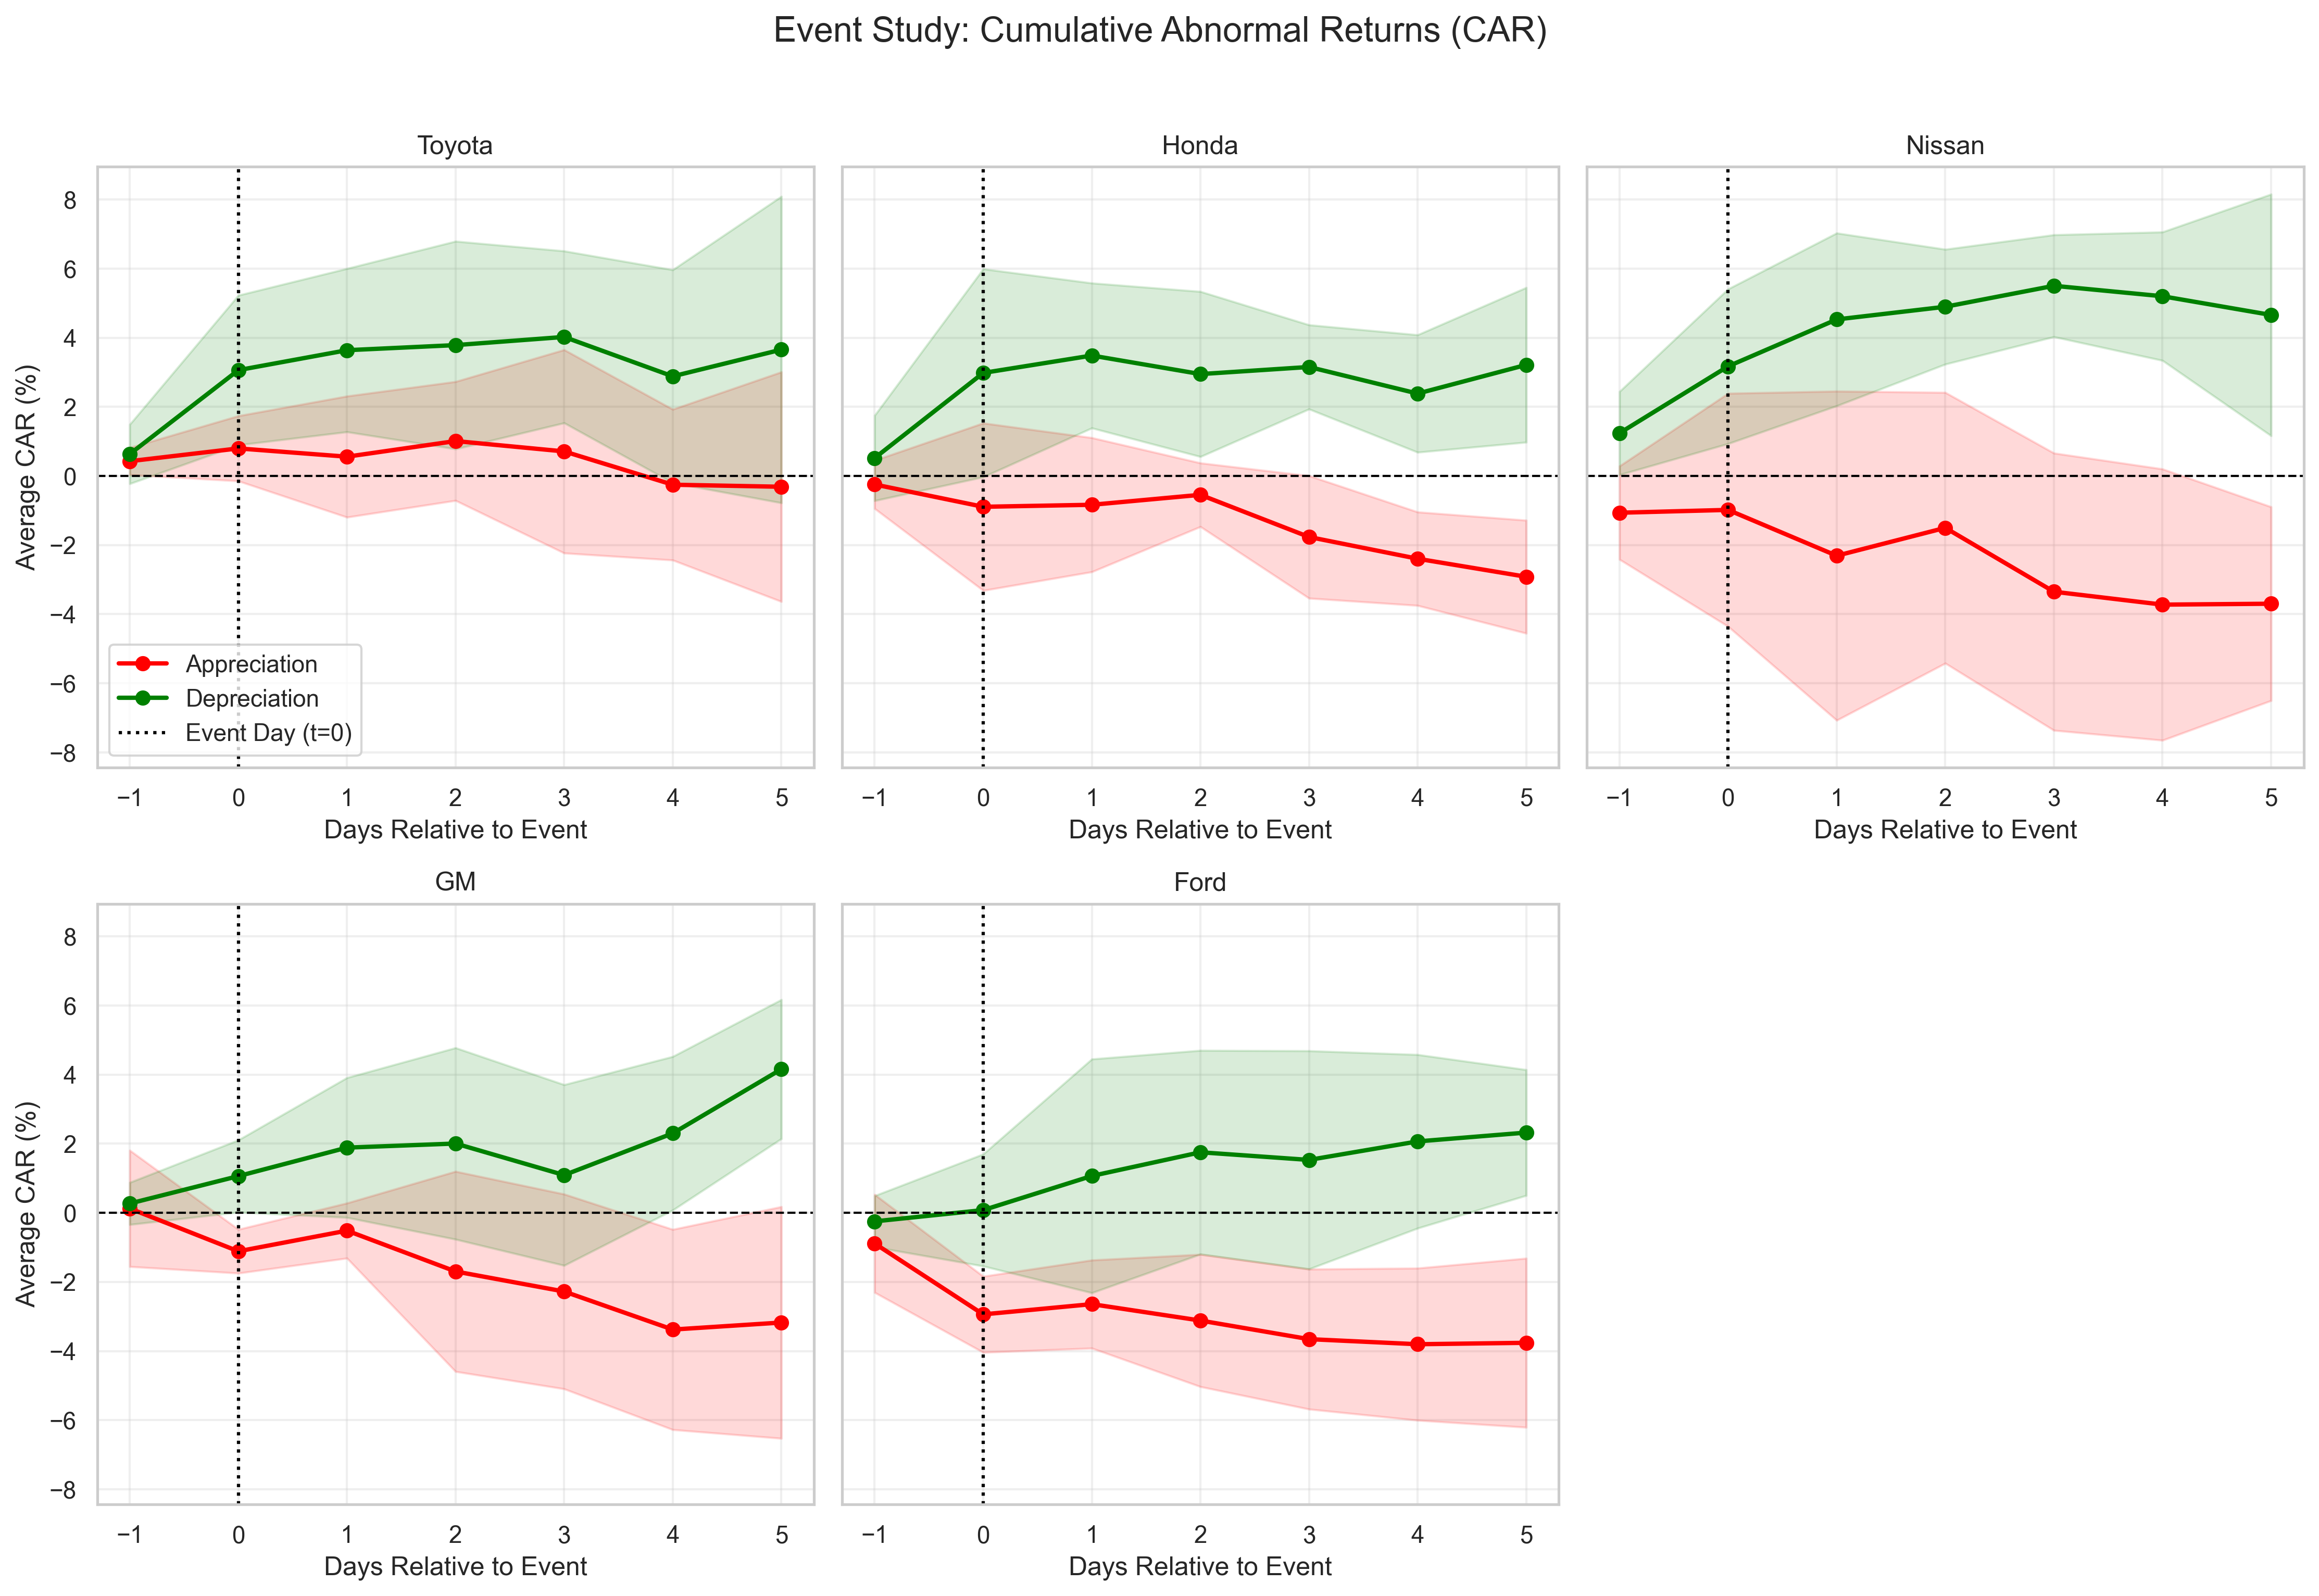
\includegraphics[width=0.9\textwidth]{event_study_car.png}
\caption{Average cumulative abnormal returns (CAR) over $[-1,+5]$ around BOJ/Fed FX-shock events, partitioned by Yen depreciation (green) and Yen appreciation (red). Shaded regions represent cross-event uncertainty bands.}
\end{figure}

Three results are central.

\paragraph{(1) Toyota's CAR is near zero under both regimes.}
Toyota's average CAR remains close to zero after Yen appreciation episodes (about $-0.31\%$ by $t=5$) and modest after depreciation episodes (about $+3.66\%$), with neither response statistically distinguishable from zero in the reported summary. This symmetry is precisely what one would expect from a firm whose operating cash flows are largely currency-matched.

\paragraph{(2) ``Sensitive cohort'' firms react strongly to Yen moves.}
Honda, Nissan, GM, and Ford display pronounced asymmetry: Yen appreciation shocks generate negative CARs, while Yen depreciation shocks generate positive CARs. In particular, Honda and Nissan exhibit sizable negative abnormal performance after appreciation episodes, consistent with profit compression and adverse translation when the Yen strengthens.

\paragraph{(3) Timing: responses build over multiple days.}
CARs typically drift over several sessions rather than jumping entirely on $t=0$. This is consistent with gradual information incorporation: policy shocks first move FX markets, then investors revise earnings expectations, and only then do abnormal returns cumulate.

\paragraph{Synthesis: linking the statistics back to trade history.}

Taken together, the LP-IV and event-study designs deliver a consistent message: exchange-rate exposure in the auto sector is real but highly firm-specific. Toyota appears to have neutralized the traditional currency channel, while other firms remain exposed.

From a historical perspective, this is not accidental. The ``trade war'' era created strong incentives for Japanese automakers to become domestic producers in the US, and the Plaza Accord transformed localization from a quota-avoidance tactic into an existential hedge against currency misalignment. Toyota's exceptional insulation today is best read as a long-run outcome of that strategic commitment.

\section{Discussion: Implications for Trade Narratives and Risk Management}

\paragraph{Rethinking the ``weak Yen advantage'' in US--Japan auto politics.}

US political debates have often treated Yen depreciation as a direct subsidy to Japanese auto exports. Our results suggest a more nuanced reality. A weaker Yen still matters for some firms---Honda and especially Nissan exhibit meaningful positive sensitivity---but it does \emph{not} uniformly advantage all Japanese automakers. Toyota, the largest and most symbolically prominent Japanese OEM, shows negligible exposure. In other words, the firm most often at the center of the US political narrative appears least affected by the exchange-rate mechanism that narrative emphasizes.

This has two interpretive implications. First, trade-policy arguments premised on a homogeneous ``Japan export model'' are increasingly outdated. Second, the effectiveness of localization as an operational hedge implies that long-run exposure is partly endogenous to past trade conflict: firms that faced the most political pressure and invested most heavily in North American production are precisely those that attenuated currency sensitivity.

\paragraph{Why localization neutralizes exposure: a cash-flow mapping.}

The simplest way to connect the statistics to economic structure is through the currency composition of operating cash flows. Let Dollar revenues from US sales be $R^{\$}$ and Dollar costs be $C^{\$}$. The net Dollar operating surplus is $\Pi^{\$}=R^{\$}-C^{\$}$. If a firm exports from Japan, $C^{\$}$ is small and $C^{\yen}$ is large, so a Yen depreciation increases $\Pi^{\yen}$ both by raising foreign revenues in Yen terms and by improving pricing flexibility. If a firm produces locally, both $R^{\$}$ and $C^{\$}$ are large, so $\Pi^{\$}$ is less sensitive to USD/JPY.

Toyota's zero response is consistent with high $C^{\$}$ relative to $R^{\$}$ for its North American business (a matched position). Nissan's large positive response is consistent with a larger unmatched component (either more Japan-based exports, more Yen-denominated cost exposure, or less ability to stabilize margins through pricing-to-market).

\paragraph{Limitations and robustness considerations.}

Two caveats are important when interpreting magnitudes.

First, the IV identifies the effect of \emph{yield-driven} exchange-rate variation. If 2-year yield shocks affect automaker equities directly through discount-rate or demand channels, the exclusion restriction could be imperfect. Controlling for the S\&P~500 mitigates broad risk-on/risk-off effects, but industry-specific interest-rate sensitivity may remain.

Second, measurement choices matter for international firms. If Japanese equities are measured via US-traded ADRs, USD/JPY movements can mechanically affect dollar-denominated returns even if the underlying Yen share price is unchanged. The fact that Honda and Nissan respond positively (rather than mechanically negatively) suggests fundamentals dominate translation in these episodes, but future work could replicate the analysis using home-market Yen prices and then explicitly decompose returns into local-equity and currency components.

A natural extension is to examine nonlinearity and regime dependence: exposure may differ in crisis periods (when the Yen behaves as a safe haven) versus expansion periods (when interest differentials dominate).

\section{Conclusion}

The US--Japan auto relationship has been shaped by a long interaction between trade conflict and currency politics. From oil-shock-driven import penetration and the early-1980s VERs to the Plaza Accord and decades of transplant expansion, policy shocks repeatedly altered the geography of production. This paper shows that those historical adjustments are visible in modern financial sensitivity.

Using LP-IV and event-study evidence, we document strong firm-level heterogeneity in exchange-rate exposure. Honda, Nissan, GM, and Ford display positive equity responses to a monetary-policy-induced USD/JPY appreciation (Yen depreciation), while Toyota is essentially insulated. The results provide a firm-level resolution to the exchange-rate exposure puzzle: exposure is not a uniform feature of ``Japanese automakers'' or ``exporters'' but an endogenous outcome of operational structure and localization.

For policymakers, the implication is that exchange-rate arguments in trade disputes should be targeted and evidence-based: the currency channel is real for some firms but close to irrelevant for others. For firms and investors, the implication is that ``macro'' risk is not only hedged in derivatives markets; it can be engineered---or eliminated---through decades of production and supplier strategy.

\bibliographystyle{apalike}

\bibliography{references}

\end{document}
